\documentclass[conference]{IEEEtran}
\IEEEoverridecommandlockouts
% The preceding line is only needed to identify funding in the first footnote. If that is unneeded, please comment it out.
\usepackage{cite}
\usepackage{amsmath,amssymb,amsfonts}
\usepackage{algorithmic}
\usepackage{graphicx}
\usepackage{textcomp}
\usepackage{xcolor}
\usepackage{colortbl}
\def\BibTeX{{\rm B\kern-.05em{\sc i\kern-.025em b}\kern-.08em
    T\kern-.1667em\lower.7ex\hbox{E}\kern-.125emX}}
\begin{document}

\title{Automatic Tweet Spam Detection Using Supervised Machine Learning Algorithms}

\author{\IEEEauthorblockN{Abdallah Kharouf}
\IEEEauthorblockA{\textit{Computer and Electrical Engineering Department} \\
\textit{Birzeit University}\\
Ramallah, Palestine \\
1183328@student.birzeit.edu}
\and
\IEEEauthorblockN{Ala Ahmad}
\IEEEauthorblockA{\textit{Computer and Electrical Engineering Department} \\
\textit{Birzeit University}\\
Ramallah, Palestine \\
1183339@student.birzeit.edu}
}

\maketitle

\begin{abstract}
The spamming problem in Twitter is one of the most critical problems in the online world. Researchers have been working hard to find effective ways to classify tweets' contents and Twitter users to spam or not spam by employing different machine learning algorithms that basically depends on the extraction of the most useful information, or attributes, from a tweet's content and a user's profile. In this paper, we dealt with a data set of classified tweets by cleaning the data with a series of preprocessing and pruning techniques to make it ready to enter a machine learning model for learning and then applied some tests to the fit models to measure their performance. 
\end{abstract}

\begin{IEEEkeywords}
spam, machine learning, algorithm, data set, preprocessing, pruning, fit model
\end{IEEEkeywords}

\section{Introduction}
Twitter is one of the most famous social media platforms which allow users to stay connected on topics and news and almost anything related to a user's life as it uses so much complex and advanced algorithms which detects the topics that interests each user to give him more and more of the content s/he likes. One of the most interesting feature in Twitter is the \textit{Hashtag}, which collects tweets that are relevant by using the hashtag symbol "\#". The concept of hashtag is easy, assume you want to share a tweet about your favourite football team, e.g Real Madrid, you share the tweet and put "\#Real\_Madrid" in it. When doing this, your tweet will be seen by anyone who searches for the same hashtag. From the hashtag concept, the concept of \textit{Trending Topics} was extended, which are the hashtags that have the most tweets in it. Controlled Users see Twitter as an opportunity for them to share their spam tweets for purposes of getting famous, sharing malicious URLs, spreading fake news, advertising products or even spreading hate speech and almost always make their spamming ways by putting their tweets in the Trending Topics section by using the famous hashtags irrelevantly of the their tweet's topic. This problem in Twitter have made lots of users uncomfortable and in danger of getting fake news, phished or getting their private data stolen by a malicious URLs or so and hence researchers and studies have been trying to find an automated way to detect spam tweets and removing them from Twitter to make users comfortable.

Researchers have found their answers in Machine Learning to classify tweets automatically. In machine learning, one needs a good study of the characteristics in which from it s/he can say that this tweet is spam or not. One of the main characteristics that were considered is that the spam tweets are unsolicited, hence they get small reactions from users such as likes, comments, retweets or favourites unlike regular users who mostly have more actions in their tweets. Other characteristics was the number of hashtags or URLs in a tweet, as a spam tweet would have much more hashtags than a regular one so the tweet would be seen in multiple trending topic. The text of the tweet also found to be a good characteristic in spam detection, as the controlled users found to use some similar words in their tweets, most of these words are the "\textit{attractive words}", such as ``Hey !!'', ``Did you know !'' and ``Watch out !!'' which attracts users to read the content of the tweet.

In machine learning, the set of characteristics that defines something is called a \textbf{\textit{Feature Vector}}. Feature Vector is one of the main blocks in machine learning and hence its attributes must be (1) independent of each other so that each attribute gives information about the classification different that the other, (2) highly correlated with the classification of the tweet, (3) contain high information in them, and (4) relevant for all other attributes such as the \textit{number of hashtag} attribute and \textit{tweet text} attribute must describe the same tweet. Furthermore, when working in a supervised machine learning model, as in the models implemented in the paper here, each vector in the feature vector must be labeled if spam, or not.

In this paper, several data pruning and preprocessing techniques will be implemented to extract the feature vector from the given data set, clean the invalid values and calculate some attributes. The rest of papers is divided as follows: Section 2 discusses previous work from researches in the field, Section 3 discusses the data processing techniques used, Section 4 discusses the learning models implemented and the final section concludes the paper and discusses results.

\section{Related Work}
In the study of Twitter spammers, many studies worked hard towards finding the best set of features that discriminate tweets and classify them as spam, or quality tweet. However, along with researchers working hard towards detecting spam tweets, controlled users and spam accounts worked even harder to bypass the researchers'  methods of detection. One of the studies on Twitter spammers, suggested that the follower's number is the biggest clue in spam detection, since a controlled user won't  have big popularity in Twitter and thus small number of followers\cite{b1}. To bypass this, controlled users now try to make their accounts popular enough to make their detection harder.

Kabakus and Kara on their survey on spam Detection methods on Twitter\cite{b2} had some interesting and informative points on methods of Account-based Spam Detectıon Methods and Tweet-based Spam Detection Methods. In Account-based Spam Detectıon, they referred to concepts such as: spammers get less likes and comments because they are unsolicited, spammers tend to post lots of tweets per day to attract attention of legitimate users, spammers tend to add lots of hashtags and URLs to their tweets to attract attention and that spammers tend to post same or similar tweets. Moreover, in Tweet-based Spam Detection Methods, they proposed concepts of detection such as: spammers use lots of mentions to legitimate and popular accounts to attract attention, spammers uses URLs in their tweet spam tweets to drive users to their websites and that spammers uses hashtags, especially the trending ones, to get more visibility.

Washaha and Qaroush tried to build a real-time model to detect spam tweets from unsupervised set of data\cite{b3}. They built a feature vector of 17 features to help with detecting spam tweets, then they boosted these 17 features by classifying them using a supervised model's output on the training tweets set, thus resulting in 18 two-dimensional matrix representing the feature vector. Their 17 features contained features related to the tweet itself, such as: number of hashtags, URLs, words, characters, mentions, replies, favourites, URLs per word and hashtags per word, and others related to the user, such as: number of following, followers, lists, tweets and the age of the account. 

Tingmin Wu and Sheng  Wen shared their study in which they compared some of the approaches in Twitter spam detection\cite{b4}. In which they analyzed methods of Syntax Analysis for the tweet body and Feature extraction from the environment of the tweet. In syntax analysis method, three main concepts were used to analyze the tweet content, these are TF-IDF, Bag-of-words and Sparse Learning. TF-IDF is the most popular technique to extract the meaning of tweets and it's used in text retrieval to obtain the representation terms and weights of contextual words, here it was used to detect tweet duplicates in a campaign and then these campaigns will be classified into spam, or quality, campaigns. Bag-of-words method was a typical text representation and was widely used for preprocessing tweets before training a classifier, here it used the output of the previous TF-IDF model to find the text-based features and calculate tweet similarity. Noted that both TF-IDF and Bag-of-words uses the assumption that spam tweets have similar content between each other. The other approach discussed here was the method of Feature extraction, in which the Cumulative Distribution Function (CDF) analysis method was taken into account to find the best feature vector to determine if the tweet is spam or not. This method calculated the statistical information in each feature from the tweet feature table and found whats the best informative feature in the table, using this, it was found that spam tweet have lots more hashtags, URLs and spam words than quality tweets.

From the study of different works in the field, we wanted to merge between methods suggested by different studies to get one stable and accurate model of classifying spam and quality tweets. Our approach will be using both the Syntax analysis and feature extraction methods together. The syntax analysis will use the Count Vector and TF-IDF concepts in Natural Language Processing to learn the tweet contents. This resulted NLP model will be used to get one more additional feature to add to the feature vector. The feature vector will have the features of Number of words, chars, digits, URLs, hashtags, mentions, followers, following, actions on tweet, ratio of followers to following, URLs to words, hashtags to words and the NLP model result from previous pipeline.

\section{Data Processing}
Data collection and processing is almost the hardest part in any machine learning project. Thus, most of the time and efforts are spent in preprocessing, pruning and cleaning of invalid data. The data provided for the paper was composed of almost 12,000 tweet, this isn't a large number in machine learning models in which they usually have more than 100,000 tweet in their data sets. Even though the number of tweets provided are small, the data is not clean and it has to be pruned.
The data of tweets is in \textbf{\textit{csv}} format, which is a format that separates attributes by comma and elements by lines. Each Tweet is represented in one line by set of attributes; \textit{Id,Tweet,following,followers,actions,is\_retweet,location,Type}. Which gives each tweet an Id, introduce its text, how many reactions it had, the number of followers and following users to the author account, the provided location of the author account and the type of the tweet; \textbf{Spam, or Quality}.

\subsection{Missing Values}

Large number of the tweets have missing attributes in them, these represent \textbf{\textit{nan}}, not a number, when reading these values into \textbf{\textit{python}}, reading null values and accessing them later will result in run exception for trying to operate on null values, also you can't create your feature vector and train your model if it had null values. However, not all missing values for any attribute matter as will be explained in the upcoming sections, only the values of \textit{Tweet,following,followers,actions,is\_retweet,Type} attributes does matter to be real values and related to the tweet itself.

Several solutions to this problems was introduced and experimented, first was to substitute the missing values with 0. However, this is not possible since this is \textbf{interval attribute} and the 0 represents a value in model's calculations, not null. Second solution was to substitute the missing values by the mean of the column of that attribute, this is a good approach, however it will provide data that is not related to the tweet itself and won't result in better model calculations, since the mean values get removed in our model for better performance.

The settled solution was to dismiss any data with one of the values from the attributes missing. In this way, you can guarantee a good and clean data, even if it became even smaller. The number of missing values for these attributes were in 2,000 tweet, and thus the data set has became smaller to almost 10,000 tweet.

\subsection{Cross Validation Method}

Since the data set is limited and there's no other resource to get additional tweets from such as real-time tweets, the data provided was divided multiple times. First, \textbf{30\%} of the data were given to train the text processing modle which will be explained later, the other \textbf{60\%} was predicted by the same model and their results were recorded to use later. Then, the same \textbf{60\%} of data that was predicted in the previous model is now divided to \textbf{80\%} to train the main machine learning model and the other \textbf{20\%} to test it, this method is called the \textbf{\textit{Cross-Validation Method}}, and it is a famous method to use when you have small data set to use for training your machine learning model and to test it.

\subsection{Features Extraction}
The process of feature extraction is divided into two modules; text processing and features analysis. The text processing module study the text of the tweet and analyse it using concepts of \textbf{Natural Language Processing} such as TF-IDF and Count Vector. Meanwhile, the feature analysis studies the attributes of the data set and chooses the most informative attributes to the tweet class.
\subsubsection{Natural Language Processing}
The process of text learning, or analysing, is grouped in a pipeline (the concept of the pipeline is explained in the next subsection), where it first starts with the Count Vector block, pass by the TF-IDF block and through the Standard Scalar to reach the \textbf{Multi-layer Perceptron} for training. The process starts first with the Count Vector, which converts the words in raw text to token count vectors, thus \textbf{\textit{Vectorizing}} the text. The second block is TF-IDF, which means term-frequency times inverse document-frequency. The goal of using TF-IDF instead of the raw frequencies of occurrence of a token in a given document resulted from the Count Vector is to scale down the impact of tokens that occur very frequently in a given corpus and hence are empirically less informative than features that occur in a small fraction of the training corpus.  figure~\ref{fig:NLP-pipeline} below shows a block diagram of the pipelining model for the text processing module.
\begin{figure}
    \centering
    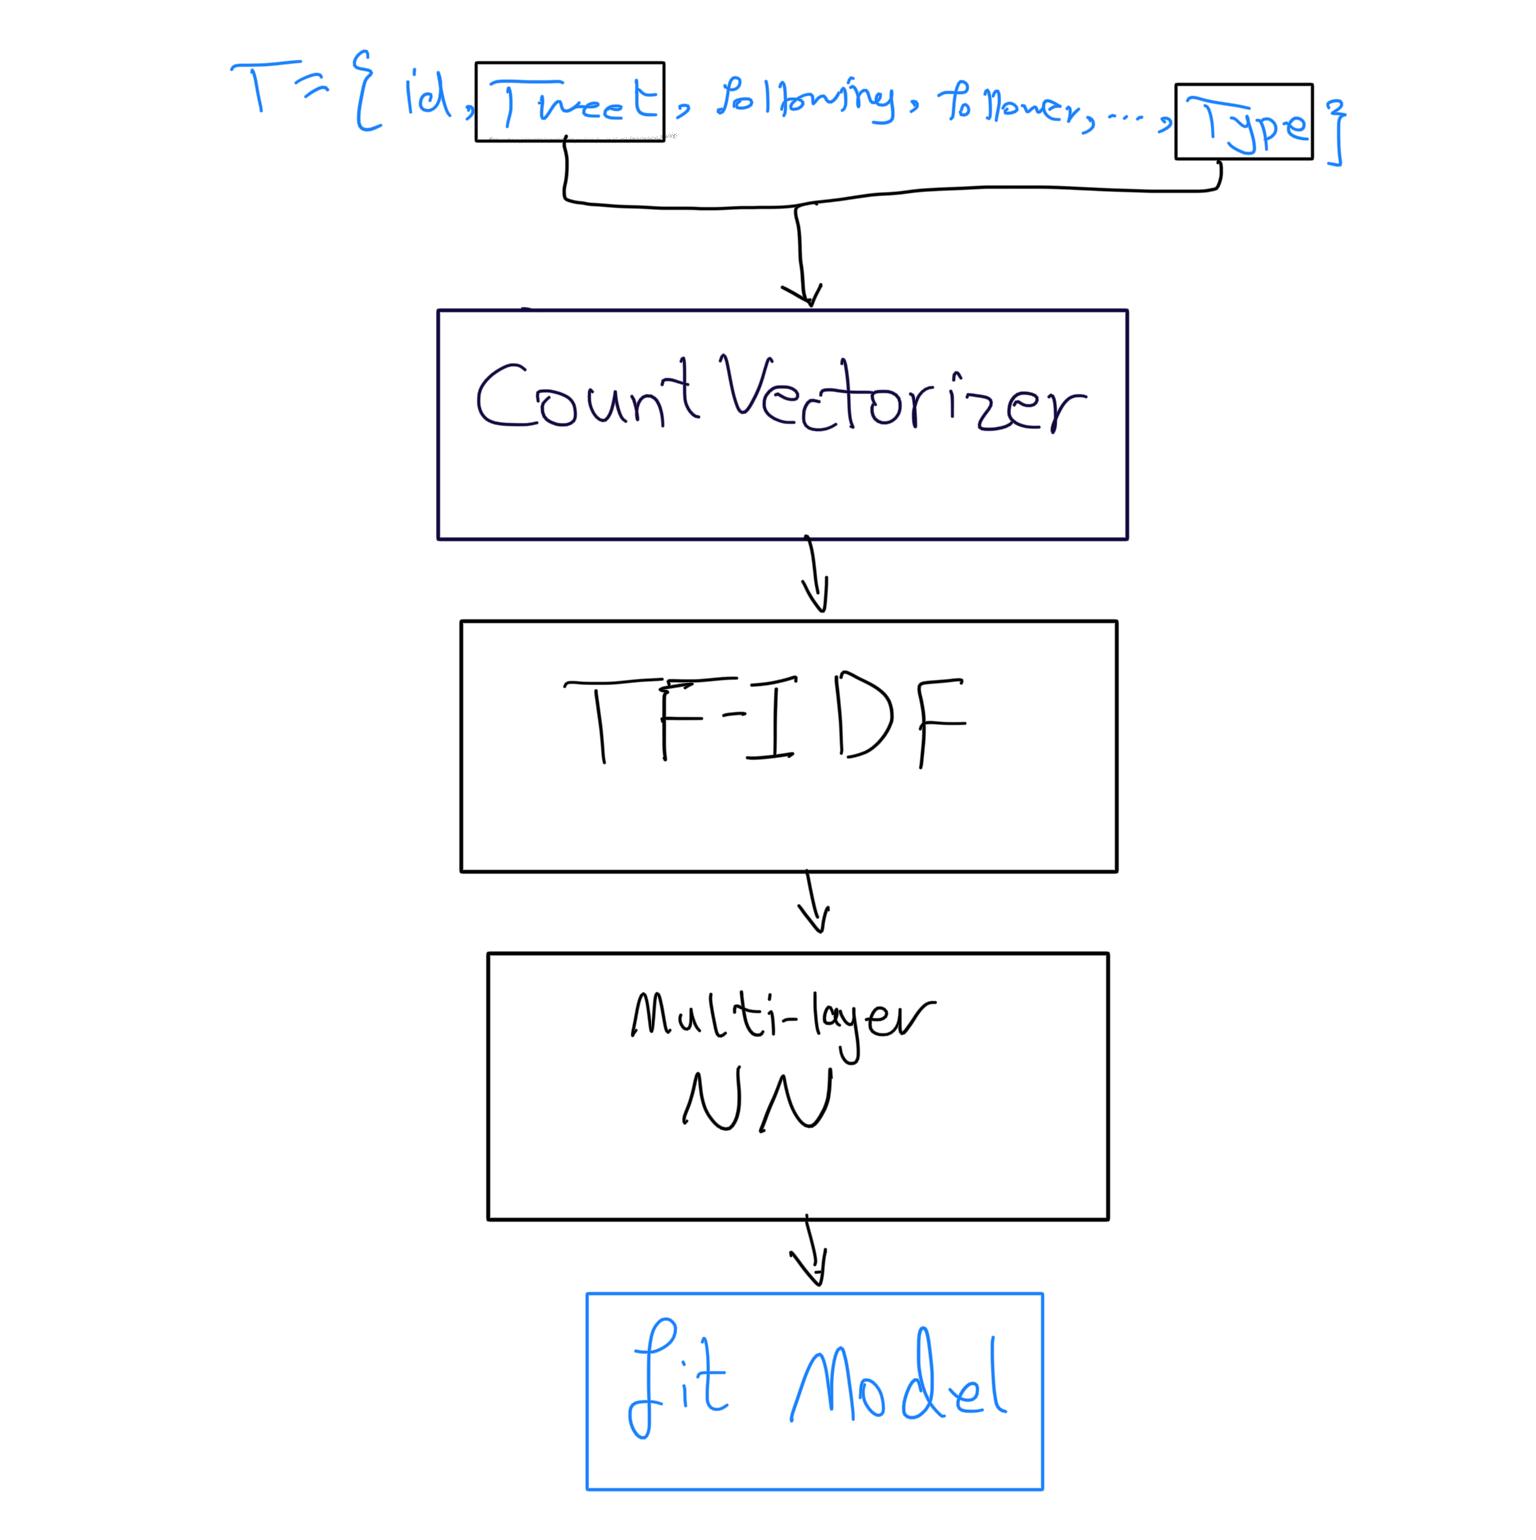
\includegraphics[scale=0.1]{NLP-pipeline.png}
    \caption{Block diagram of text processing pipeline}
    \label{fig:NLP-pipeline}
\end{figure}

\subsubsection{Features Analysis}
To make use of the good attributes provided in the data set, the method of feature extraction were used too. This method uses some useful attributes of the tweet that are provided in the data set or calculated from other attributes to create a useful feature vector to model in the main machine learning model. The selected features were as shown in table~\ref{table:feature-vector}. The correlation of each feature with the target value (Spam, or Quality) is important, since this correlation indicates that the feature gives useful information about the tweet classification. Moreover, if two features are highly correlated, one of them must be dropped since they give the same information about the target value of classification. Correlation $r$ between two features are calculated by the Person's equation defined below.

\begin{equation}
    r = \frac{{}\sum_{i=1}^{n} (x_i - \overline{x})(y_i - \overline{y})}
{\sqrt{\sum_{i=1}^{n} (x_i - \overline{x})^2(y_i - \overline{y})^2}}
\end{equation}

where $\overline{x}$ is the mean value of feature $x$ and $\overline{y}$ is the mean value of feature $y$. figure~\ref{fig:corr-matrix} shows the correlation between the features in the feature vector. Note that most of the features have small correlation between them or even no correlation, hence they're good to use. However, some features have large correlation between them, these will be eliminated using techniques that will be used next, i.e.  \textbf{$\chi^2$ method} that will be explained next.

\begin{table}
\centering
\caption{Attributes of the feature vector}
\label{table:feature-vector}
\begin{tabular}{|l|l|} 
\hline
\rowcolor[rgb]{0.753,0.753,0.753} Feature         & Description                                        \\ 
\hline
\rowcolor[rgb]{0.753,0.753,0.753} no\_word        & Number of words in tweet                           \\ 
\hline
\rowcolor[rgb]{0.753,0.753,0.753} no\_char        & Number of chars in tweet                           \\ 
\hline
\rowcolor[rgb]{0.753,0.753,0.753} no\_digit       & Number of digits in tweet                          \\ 
\hline
\rowcolor[rgb]{0.753,0.753,0.753} no\_hashtag     & Number of hashtags in tweet                        \\ 
\hline
\rowcolor[rgb]{0.753,0.753,0.753} no\_usermention & Number of usermentions in tweet                    \\ 
\hline
\rowcolor[rgb]{0.753,0.753,0.753} no\_url         & Number of URLs in tweet                            \\ 
\hline
\rowcolor[rgb]{0.753,0.753,0.753} no\_following   & Number of following accounts for the tweet author  \\ 
\hline
\rowcolor[rgb]{0.753,0.753,0.753} no\_follower    & Number of followers to the tweet author            \\ 
\hline
\rowcolor[rgb]{0.753,0.753,0.753} reputation      & Ratio of followers to following                    \\ 
\hline
\rowcolor[rgb]{0.753,0.753,0.753} actions         & Actions on the tweet (favorites, replies, etc.)    \\ 
\hline
\rowcolor[rgb]{0.753,0.753,0.753} url\_word       & Ratio of URLs to words in tweet                    \\ 
\hline
\rowcolor[rgb]{0.753,0.753,0.753} hashtag\_word   & Ratio of hashtags to words in tweet                \\ 
\hline
\rowcolor[rgb]{0.753,0.753,0.753} nlp\_result     & Result of the text processing model                \\
\hline
\end{tabular}
\end{table}

\begin{figure}
    \centering
    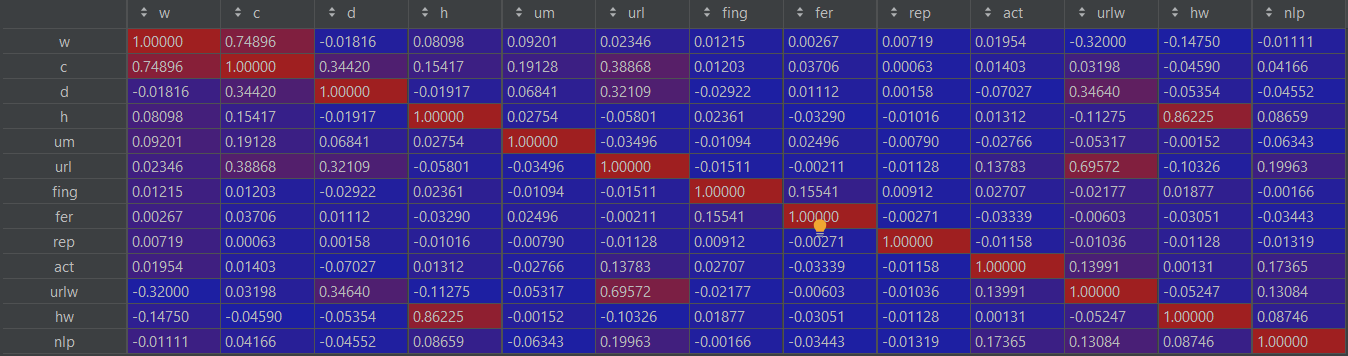
\includegraphics[scale=0.3]{correlation-matrix.png}
    \caption{Correlation matrix for the features in feature vector}
    \label{fig:corr-matrix}
\end{figure}

\subsection{Pipelining Data}
To work with data in more efficient and effective way, a pipeline module was used. The pipeline module basically forces the data to go in a series of processing tools in such a way that a block output is an input to another block. The first block in the pipeline is the \textbf{Variance Threshold} block, this block receives the data after reading it from the \textbf{\textit{csv}} file and deleting the missing values and then it processes it by removing the columns (attributes) where the variance exceeds \textbf{80\%}. The variance is a measure of the values similarity in all the columns, and is calculated by the equation 

\begin{equation}
Var(x)=p(x)(1-p(x))
\end{equation}
where $p(x)$ is the probability of the attribute $x$ .

The second block in the pipeline is the \textbf{$\chi^2$ Statistic}, in which the attributes that are not relative to the output class are removed, as the chi-square test measures dependence between stochastic variables, and is calculated by the equation

\begin{equation}
\chi^2 = \sum \frac{(O_i – E_i)^2}{E_i}
\end{equation}
where $O_i$ is the observed value and $E_i$ is the expected value of an attribute's value.

The third block in the pipeline is the \textbf{Standard Scalar}, which is one of the ways of standardization of the data set, which is a common requirement for many machine learning estimators. The block ignores the shape of the distribution in a column and just transform the data to center it by removing the mean value of each feature, then scale it by dividing non-constant features by their standard deviation. The standard score of a sample $x$ is calculated by the equation

\begin{equation}
z = \frac{(x - u)}{s}
\end{equation}

where $u$ is the mean of the training samples and $s$ is the standard deviation of the training samples.

After the data is processed through the three blocks of the pipeline, it is considered ready and suitable to enter a machine learning model to train in it. The machine learning model is the last block of the pipeline, it accepts the input coming out of the \textbf{Standard Scalar} and produces a fit model. Figure~\ref{fig:feat-pipeline} visualizes the process of the pipeline explained in a block diagram.

\begin{figure}
    \centering
    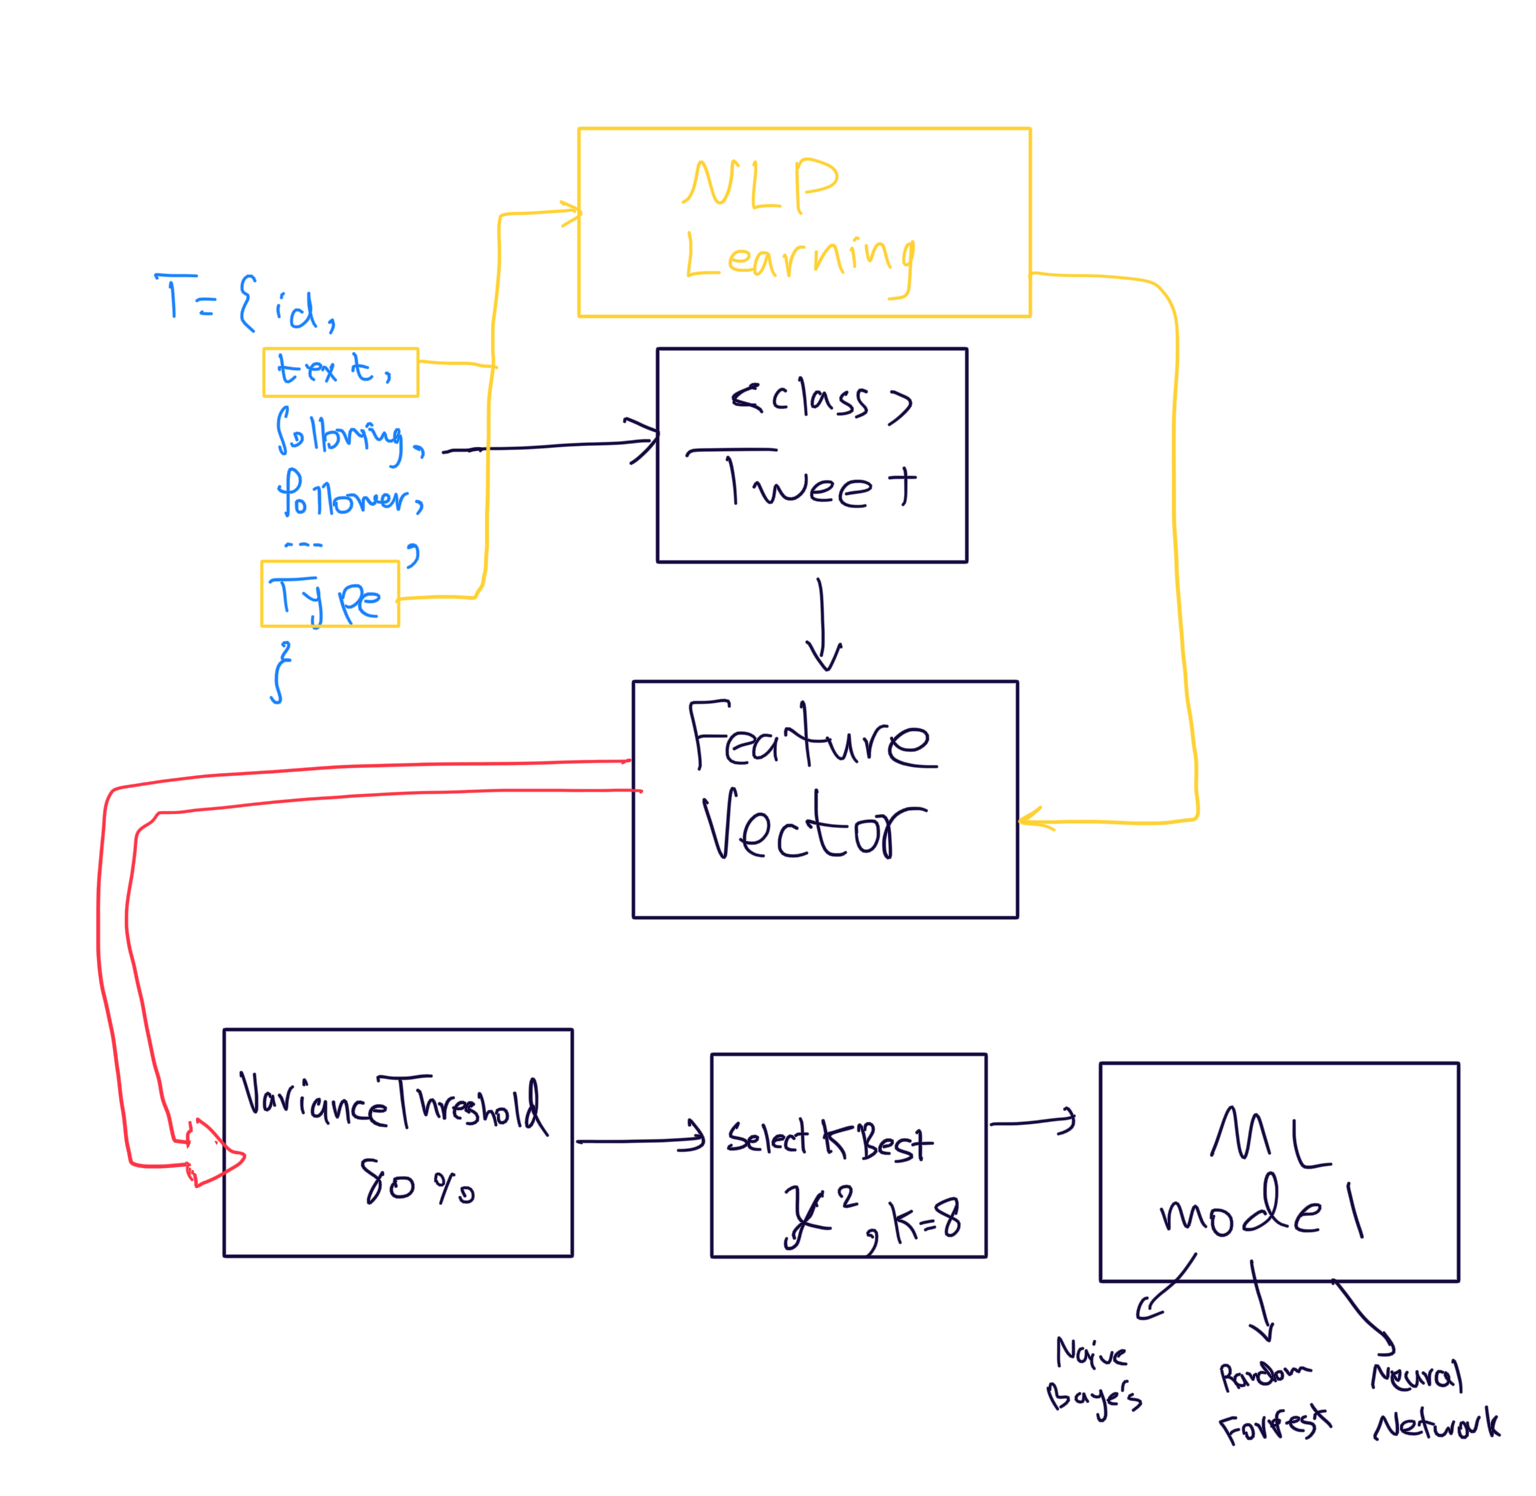
\includegraphics[scale=0.1]{feature-pipeline.png}
    \caption{Block diagram of feature analysis pipeline}
    \label{fig:feat-pipeline}
\end{figure}

\section{Learning}
Different machine learning models were used to learn the feature vector extracted from a prior series of data pruning, data preprocessing and text learning along with feature extraction from the raw data which were done in a pipeline of multiple transformations, the last block of the pipeline is the machine learning model that will be trained by that data. The main goal of using different models in learning is to compare their performance and ability to fit a good function from the \textit{hypothesis space} for future use of prediction. Three main models of machine learning algorithms were used; \textbf{Naïve  Bayes Classifier}, \textbf{Random Forrest algorithm} and \textbf{Multi-layer Perceptron}. The models will be compared by their confusion matrices, accuracy, precision, recall value and F1 value.  

\subsection{Naïve  Bayes}
Naïve  Bayes theorem tries to find the probability of an event to occur based on the probabilities of prior events based on equation~\ref{eq:nb}. In the case of tweets classification, this model tries to predict the probability of a tweet to be Spam or Quality with the set of feature vector $F$ based of prior knowledge of each feature's probability to happen in the learning phase of the model. The model was used to fit the train data of tweets and its scored were measured from the test data as shown in table~\ref{table:nb-res}

\begin{equation}
p(y|X) = \frac{p(X|y)p(y)}{p(X)}
    \label{eq:nb}
\end{equation}

\begin{table}
\centering
\caption{Naïve Bayes Model Results }
\label{table:nb-res}
\begin{tabular}{|c|c|c|c|l|l|l|l|} 
\hline
\rowcolor[rgb]{0.753,0.753,0.753} Accuracy & Precision & Recall & F1   & \multicolumn{4}{l|}{Confusion Matrix}  \\ 
\hline
\rowcolor[rgb]{0.753,0.753,0.753} 73\%     & 70\%      & 98\%   & 82\% & 117 & 319 & 9 & 767                    \\
\hline
\end{tabular}
\end{table}

\subsection{Random Forrest}
Random Forrest is the algorithm which tries to build multiple decision trees based on random selection from the learning split of the data set. The multiple trees each gives a prediction when trying to predict a certain value and the algorithm chooses the best prediction based on votes. The randomness and multi-level predictions in the algorithm works well in preventing over-fitting and thus boosting accuracy. In the case of tweet classification, the algorithm builds several trees in which each is different from the other regarding the path and the importance of each feature in the feature vector. The main equation of building a tree is the information theory of each feature, or the entropy, which described in the equation~\ref{eq:entropy}.

\begin{equation}
    H(x) = \sum p(x_i) \log_2 p(x_i)^{-1}
    \label{eq:entropy}
\end{equation}

When teaching the model through the learning data set and then measuring its score with the testing data set, the values in table~\ref{table:rf-res} shows. The model was used with $10$ generated trees and a minimum samples per split for tree of $1000$ sample, or feature vector.

\begin{table}
\centering
\caption{Random Forrest Model Results }
\label{table:rf-res}
\begin{tabular}{|c|c|c|c|l|l|l|l|} 
\hline
\rowcolor[rgb]{0.753,0.753,0.753} Accuracy & Precision & Recall & F1   & \multicolumn{4}{l|}{Confusion Matrix}  \\ 
\hline
\rowcolor[rgb]{0.753,0.753,0.753} 99\%     & 99\%      & 99\%   & 99\% & 436 & 0 & 2 & 774                      \\
\hline
\end{tabular}
\end{table}

\subsection{Multi-layer Perceptron}
Multi-layer Perceptron is the model which tries to build a linear discriminator in a space of non-linear mapped data, or inputs based on equation~\ref{eq:mnn}. Several algorithms are used to train this model, one of the most famous is the \textit{Back Propagation Algorithm} which has the main concept of propagating the error between the actual and expected values from the output neuron backward to the input neuron passing by hidden mid-neurons, this error propagation affects the weight of each neuron by \textbf{learning rate constant $\alpha$} using the \textbf{chain rule} thus producing a more fit model on every feature vector evaluated.

\begin{equation}
    h_1 = Act(\sum w_i x_i + bias)
    \label{eq:mnn}
\end{equation}

where $h_1$ is the output of a neuron, $Act$ is the activation function used, $w_i$ is the assigned weight of the neuron and $x_i$ is the input of the neuron and the $bias$ is the bias unit for the neuron.

When the model was used to classify tweets in the test set based on their feature vectors after it has learned from tweets' feature vector in the training set, interesting scores came out as shown in table~\ref{table:mnn-res}. The model was used in the Back Propagation Algorithm with 5 hidden layers with $(7, 6, 5, 4, 3)$ neuron in each level and a learning rate $\alpha=1.5e^{-5}$.

\begin{table}
\centering
\caption{Multi-layer Perceptron Model Results}
\label{table:mnn-res}
\begin{tabular}{|c|c|c|c|l|l|l|l|} 
\hline
\rowcolor[rgb]{0.753,0.753,0.753} Accuracy & Precision & Recall & F1   & \multicolumn{4}{l|}{Confusion Matrix}  \\ 
\hline
\rowcolor[rgb]{0.753,0.753,0.753} 98\%     & 98\%      & 98\%   & 99\% & 428 & 8 & 14 & 726                     \\
\hline
\end{tabular}
\end{table}

Each model has a calibration plot which measures how close the model was to detect the right function from the \textit{hypothesis space}. The calibration plot for the three learning models tried is shown in the figure~\ref{fig:cab}. The plot shows that the Multi-layer Perceptron and the Random Forrest classifiers was the most close in detecting the right function. However, the Naïve Bayes classifier didn't behave quite as well. Another way to compare the models is by studying the scores shown in tables~\ref{table:nb-res},~\ref{table:rf-res} and~\ref{table:mnn-res} which also shows that the Multi-layer Perceptron and the Random Forrest classifiers predicted values with high accuracy in opposite of Naïve Bayes which did well, but not as the others.

\begin{figure}
    \centering
    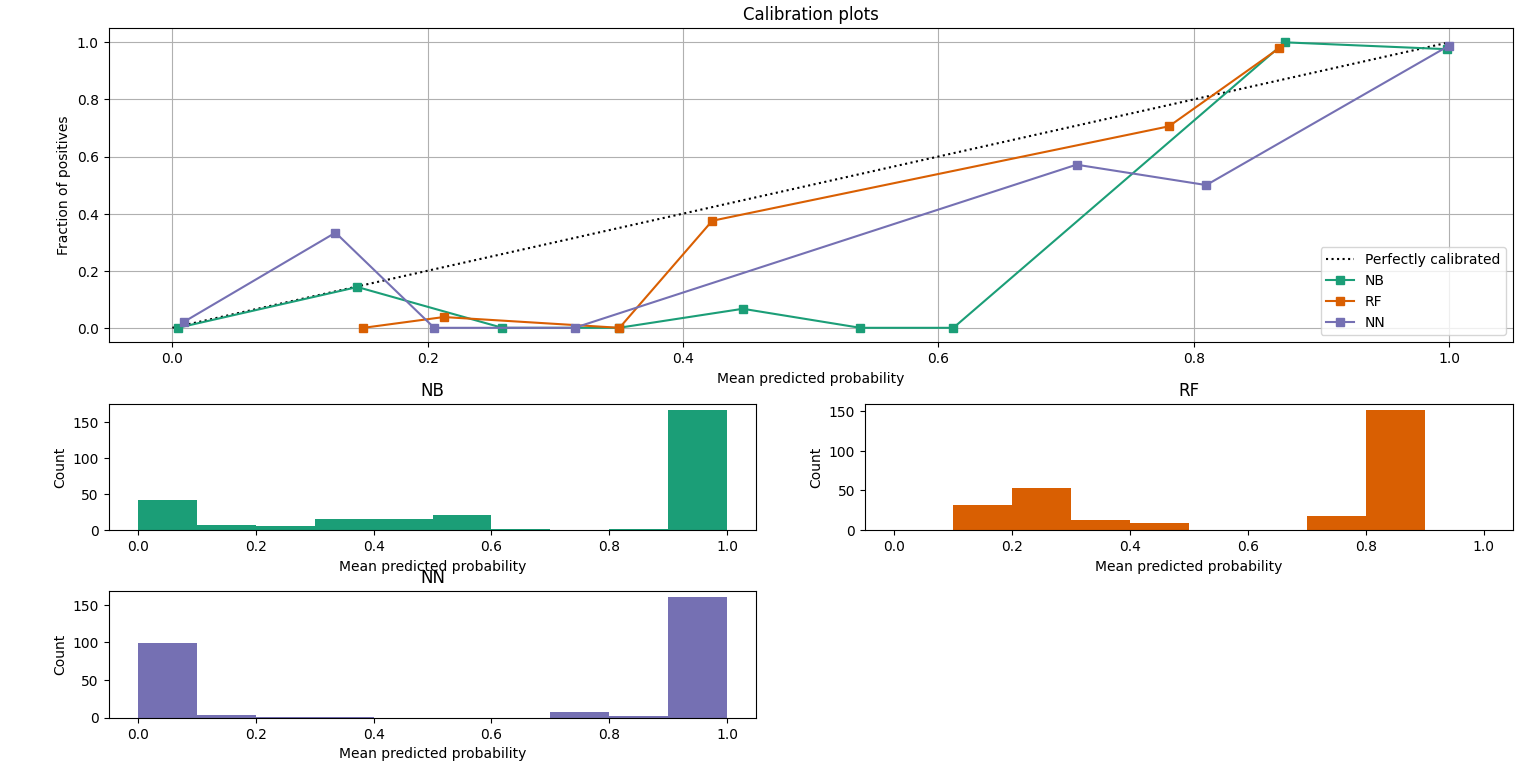
\includegraphics[scale=0.2]{calibration-plot.png}
    \caption{Calibration plot for learning models}
    \label{fig:cab}
\end{figure}

\section{Conclusion}
In this paper we tried to process the data set of previously classified tweets with their attributes by applying techniques of pruning, preprocessing and text processing to extract some of the most informative attributes to encapsulate them in a feature vector that was used in training learning models. Different learning models were implemented and trained using the extracted feature vector, we recorded their results and checked their performance to see which one is the best to use in the field.

\begin{thebibliography}{00}

\bibitem{b1} C. Chen, J. Zhang, X. Chen, Y. Xiang and W. Zhou, "6 million spam tweets: A large ground truth for timely Twitter spam detection," 2015 IEEE International Conference on Communications (ICC), 2015, pp. 7065-7070, doi: 10.1109/ICC.2015.7249453.
\bibitem{b2}Kabakus, Abdullah Talha, and Resul Kara. "A survey of spam detection methods on Twitter." International Journal of Advanced Computer Science and Applications 8.3 (2017): 29-38.
\bibitem{b3}Washha Mahdi, Qaroush Aziz, Mezghani Manel, Sedes Florence. (2019). Unsupervised Collective-based Framework for Dynamic Retraining of Supervised Real-Time Spam Tweets Detection Model. Expert Systems with Applications. 135.10.1016/j.eswa.2019.05.052. 
\bibitem{b4}Tingmin Wu, Sheng Wen, Yang Xiang, Wanlei Zhou, Twitter spam detection: Survey of new approaches and comparative study, Computers Security, Volume 76, 2018, Pages 265-284, ISSN 0167-4048, https://doi.org/10.1016/j.cose.2017.11.013.
\bibitem{b5}Al-Janabi, Mohammed, Ed de Quincey, and Peter Andras. "Using supervised machine learning algorithms to detect suspicious URLs in online social networks." Proceedings of the 2017 IEEE/ACM International Conference on Advances in Social Networks Analysis and Mining 2017. 2017.
\end{thebibliography}
\vspace{12pt}
\end{document}
